
\begin{figure*}[hbt]
\centering
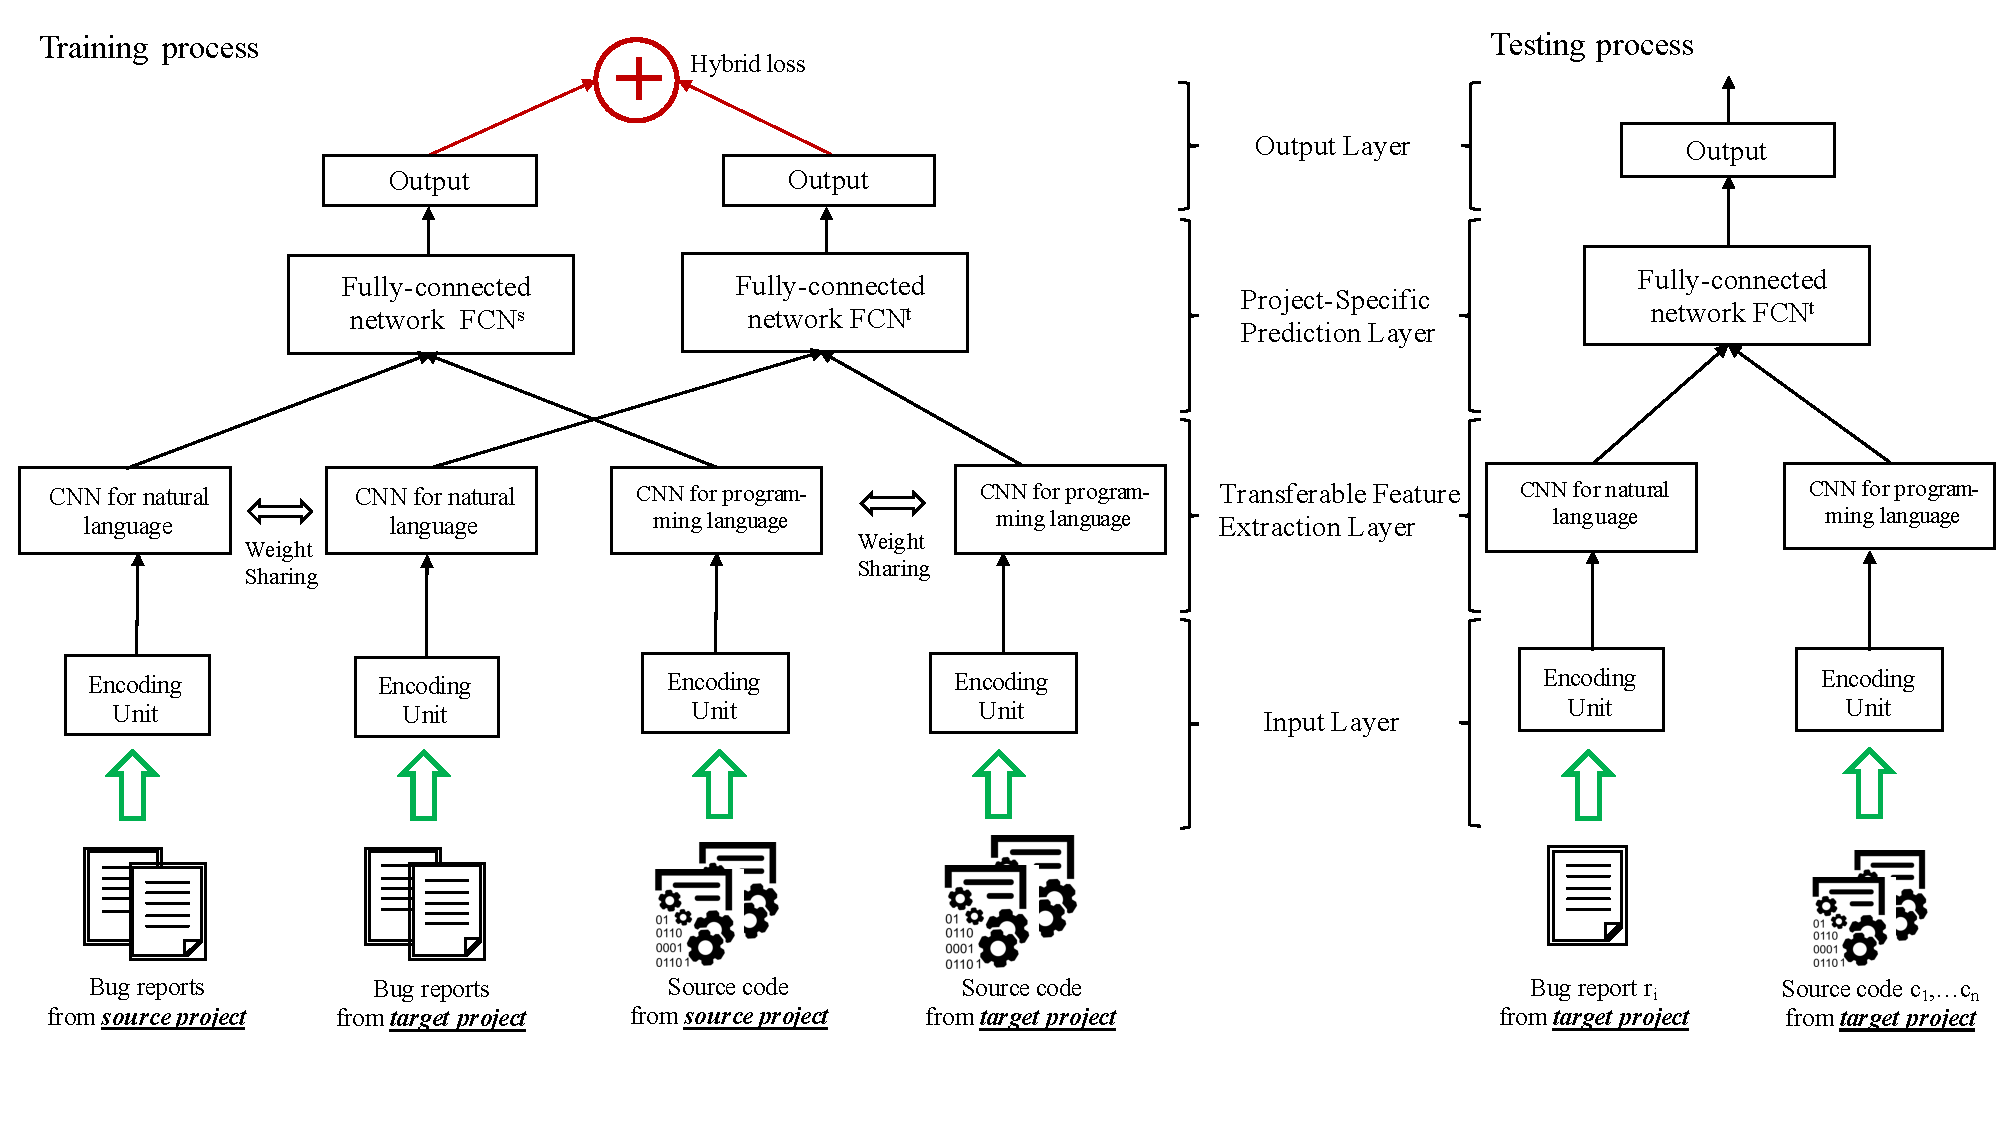
\includegraphics[width = 2\columnwidth]{pic/structure.pdf}
\caption{The overall structure of Transfer Natural and Programming language CNN.  The left part is the training process of \TRANPCNN based on the bug reports and source code from source projects and a few data from target projects, the weights of which are trained by minimizing the loss of ensemble loss from fully-connected networks $fc_s$ and $fc_t$. The right part is the testing process, a new bug report and its candidate source code are fed into the model, and \TRANPCNN outputs their relevant scores for bug localization.}
\label{fig:structure}
\end{figure*}

In cross-project bug localization, we are provided with a \emph{source} project with many bug reports carefully localized to the corresponding source code, and a \emph{target} project in which only several bug reports are localized. The goal is to construct a model to fully leverage rich information from the source project to facilitate effective bug localization for the target project.

Let $\mathcal{C}^s = \{ { c^s_1, c^s_2}, \cdots, c^s_{n^c_1} \} $ and $\mathcal{C}^t =\{ c^t_1, c^t_2, \cdots, c^t_{n^c_2} \}$ denote the set of source code files from the source project and the target project, respectively, and $\mathcal{C}=\mathcal{C}^s \bigcup \mathcal{C}^t $. Let $\mathcal{R}^s =\{r^s_1, r^s_2, \cdots, r^s_{n^r_1}\}$ and $\mathcal{R}^t =\{ r^t_1, r^t_2, \cdots, r^t_{n^r_2}\}$ denote the set of bug reports from the source project and target project, respectively, and $\mathcal{R}=\mathcal{R}^s \bigcup \mathcal{R}^t $. In the above notations, $n^c_1, n^c_2, n^r_1, n^r_2$ denote the number of source files and bug reports from source project and target project, respectively. We formulate cross-project bug localization as a learning task which aims to learn prediction functions $\mathbf{f}=(f^s,f^t)$, where $f^\alpha: \mathcal{R}^\alpha \times \mathcal{C}^\alpha \mapsto \mathcal{Y}^\alpha$. $y^\alpha_{ij} \in \mathcal{Y}^\alpha = \{+1, -1\}$ indicates whether a source code $c^\alpha_j \in \mathcal{C}^\alpha $ is relevant to a bug report $r^\alpha_i \in \mathcal{R}^\alpha$, and $\alpha \in \{s,t\}$.   % ******  typos corrected by Ming

Source and target projects may differ from each other in the way how a bug report is localized to the corresponding source code files. To effectively learn the prediction function for a target project, one problem should be addressed carefully: how to identify information from a source project that is potentially useful for learning the prediction function for the target project? Intuitively, if information from the source project can be used for the target project, both must share latent commonalities. Differences observed in the two projects are due to the way these latent commonalities are manifested. Therefore, we argue that the construction of a model that facilitates an effective cross-project bug localization can be decomposed into the two consecutive steps: 1) learning a shared latent feature representation from both source and target project, and 2) biasing the learner towards specific project considering the shared latent feature representation.   % ******  Eidited a little bit by Ming

We realize the aforementioned idea by proposing a novel deep transfer neural network named \TRANPCNN (TRAnsfer Natural and Program Language Convolutional Neural Network). Firstly, \TRANPCNN takes bug reports and source code files as inputs and learns a common transferable latent feature representation shared by both source and target projects. Next, \TRANPCNN  creates a pair of prediction functions that are biased towards the source and target project, respectively, based on the shared feature representation. 

Note that each prediction function are jointly learned with the shared transferable latent feature representation, and thus, the learning of the prediction function for either the source project or the target project is eventually beneficial for learning of the transferable features.  By employing such learning strategy, \TRANPCNN can simultaneously leverage the sufficiently large amount of well-localized data from the source project to help learning better transferable latent features and the limited number of well-localized data from the target project to adapt the shared transferable features to generate well-performing localization for the target project, which eventually overcome the data insufficiency in the target project by leveraging the sufficient localized bug reports and source codes from the source project.  % ******** Added

\ml{David and Ferdian, please help to read this part to see whether you have got the idea of learning prediction function for the source project.}




\subsection{Model Structure}

The model structure of \TRANPCNN is depicted in Figure~\ref{fig:structure}, where the subfigure to the left depicts the training process of \TRANPCNN, and the one to the right depicts the corresponding test process.

%I do not fully understand these phrases and at the moment I put them here:
%such that the common knowledge shared by both source project and the target project which can eventually facilitate the identification of the correlation between the bug report and the source codes;
%based on the fitted correlations in the source domain and the target domain, respectively

\TRANPCNN consists of four layers: input layer, transferable feature extraction layer, project-specific correlation fitting layer and output layer. The input layer takes bug reports as well as the source code files in their original formats and generate their corresponding encodings such that they can be further processed by the subsequent layers of \TRANPCNN. The transferable feature extraction layer aims to learn an intermediate latent feature representation from the bug reports and source code files shared by source and target projects.  The project-specific prediction layer is responsible for biasing learning, based on the transferable feature representation learned in the previous layer, to identify project-specific correlation patterns between bug reports and source code files in source and target projects. The output layer generates the final correlation scores for report-file pairs (i.e., pairs of bug reports and source code files). It is obvious that the the transferable feature extraction layers and project-specific prediction layer layer are the key parts of the proposed model, which would be explained in details in the following subsections. %******* Edited a little bit by Ming

\ml{Now we use ``project-specific prediction layer". But sometimes, prediction is the final output, and here we in fact output the predicted correlation scores. Other alternative here maybe ``project-specific correlation identification layer" or ``project specific localization generation layer''. Which one do you think is better?}

To train \TRANPCNN model, pairs of bug reports and source code files from the source and target projects along with their ground truth labels (i.e., correlated or not) are fed into the proposed deep model in order to learn the transferable latent feature representation shared by both source and target projects as well as the project-specific prediction functions for the source and target project, respectively. After the model is fully trained, prediction function $f^{t}$ would be used for determine the correlation of each report-file pair $(r_i^t, c_j^t)$ from the target project.

\subsection{Transferable Feature Extraction Layer}

When provided with bug reports and source code files from source and target projects in their original format, the encodings for the bug reports and the source codes are first generated by the input layer. Traditional TF-IDF (term frequency - inverse document frequency) representation~\cite{christopher2008introduction} fails to capture correlation between terms. Thus, we employ word2vec~\cite{abs-1301-3781} encoding to represent both bug reports and source code files with the purpose of enriching the initial representation, based on which, the transferable features are further extracted.

The transferable features for bug reports and source codes files should satisfy the following properties. First, the transferable features should be able to represent the functional semantics in both bug reports and source code files such that the semantics can be further utilized to identify the correlation patterns between the reports and the files. Second, the extracted semantics should be able to capture some common knowledge between the source and target project such that knowledge learned from the source project can eventually be transferred to facilitate learning for the target project.

To allow for effective knowledge transfer between source and target projects, a key challenge here is how to identify what information is useful and transferable and what is useful but may not be transferable. To address this challenge, we employ a special strategy we refer to as \emph{weight sharing} during the learning process, which imposes a hard constraint that the learned weights in the networks (both N-CNN and P-CNN) for the target project should be exactly the same as the learned weights in the networks for the source project. By weight sharing, the learning procedure that optimizes for good bug localization performances on both source project and target project is forced to focus on common features shared by both source and target projects rather than extracting project-specific features for each project. Thus, the resulting features allow for \emph{transfer} of common knowledge that is useful to determine correlation between bug reports and source code files from the source project to the target project.
 

%I'm not sure of the following sentence but the paragraph seems okay without it ... I'm not sure ...
%Note that such knowledge may need a large amount of labeled training data to be learned for any single project, but now can be directly used for the target project where the labeled training data may be limited especially for the code start.

\subsection{Project-Specific Prediction Layer} % The whole sectin is revised.

After being processed by the transferable feature extraction layers, bug reports (as well as the source code files) from both source and target project are represented using the \emph{same} set of transferable features embedded with common knowledge shared by both source and target projects.


However, since the source project and target projects may differ in the way how bug reports and source code files are correlated, the subsequent project-specific prediction layer is responsible to learn the project-specific correlation patterns considering the same set of transferable features.

Specifically, we utilize two fully-connected networks sharing the same input from the transferable feature extraction layer, namely FCN$^s$ and FCN$^t$, to learn the correlation patterns between the bug report and the source code files for both source and target projects, based on which the final prediction of correlation score is generated in the proceeding output layer. As mentioned before, learning the correlation patterns for the source project can leverage the rich supervision of the localized report-file pairs in the source project in helping the learning good transferable features, which can be conceptually regarded as pushing the useful knowledge for localizing bugs from the source project down to the transferable latent features and transferred to the target project when learning correlation patterns for the target project based on the shared latent features. 

\dl{Why do we want simultaneously learn two prediction functions? Why not just learn for target project? I'm not fully sure here ...}
\ml{Hopefully the previous paragraph addresses david's conerns.}

To jointly learn the project-specific correlation patterns for each project along with the transferable latent features, we propose the a hybrid loss function that simultaneously fulfill the learning objectives for both source and target projects. 

%Let $\varphi^{s}_{i}$ and $\psi^{s}_{j}$ denote the transferable features learn from a report-file pair $(r^s_i, c^s_j)$ with its correlation label $y^s_{ij}$ from the source project and $\varphi^{t}_{i}$ and $\psi^{t}_{j}$ with its correlation label $y^t_{ij}$ from the target project, respectively. Let $\mathbf{W} = [W_{CNN}, W_{FCN}}$ denote all the weights to be learned for the entire




%$\mathcal{L}$ is the square loss, $\lambda$ is the trade-off parameter and the weight vectors $W$ contains the weight vectors in convolutional neural networks $W_{conv}$, in fully-connected network of source domain $W_{fc_s}$ and in fully-connected network of target domain $W_{fc_t}$.

%The key challenge here is how to simultaneously learn two prediction functions capturing the correlation patterns in different project based on the same set of features within the same model structure. To address this challenge, we construct two fully connected neural network substructures, namely $fc^s$ and $fc^t$, for the subsequent project-specific correlation fitting layers, where $fc^s$ and $fc^t$ share the same input unit and have different output units. Such a special design facilitates the model to take the same set of transferable features from both bug reports and source code files and fit to correlation pattern of the report-code pair in the source project and target project, respectively, with different substructures $fc^s$ and $fc^t$.

\dl{The following phrase is unclear to me: fit to correlation pattern of the report-code pair in the source project and target project, respectively, with different substructures $fc^s$ and $fc^t$.}
\dl{I'm not sure how to fit network substructures to correlation patterns? Do we mean we use the substructures to *learn* different correlation patterns?}

%In order to fit the two network substructures $fc^s$ and $fc^t$ to different correlation patterns within the same model structure, we propose the following hybrid loss function to unify the loss from different goals into one function:
%
\begin{equation}
\begin{aligned}
\label{eq:lossfunction}
\mathop{\arg\min}_{\mathbf{w}}&\sum_{s_i,s_j}\mathcal{L}(\mathbf{h}^s_i,\mathbf{h}^s_j
,y^s_{ij}; \mathbf{w}^s_{fc}, \mathbf{w}_{conv} )\\
+&\sum_{t_i,t_j}\mathcal{L}(\mathbf{h}^t_i,\mathbf{h}^t_j,y^t_{ij};\mathbf{w}^t_{fc}, \mathbf{w}_{conv})+\lambda||\mathbf{w}||^2
\end{aligned}
\end{equation}

where, the weight vectors $\mathbf{w}=(\mathbf{w}_{conv},\mathbf{w}^s_{fc},\mathbf{w}^t_{fc})$, $w_{conv}$ is the weight vectors in convolutional neural networks, and $\mathbf{w}^s_{fc}$ is the weight in fully-connected network of source domain and $\mathbf{w}^t_{fc}$ is the weight in fully-connected network of target domain. $(\mathbf{h}^s_i, \mathbf{h}^s_j, \mathbf{h}^t_i, \mathbf{h}^t_j)$ indicates the generated middle-level features of source code and bug reports from source domain and target domain, respectively. $y^s_{ij}$ and $y^t_{ij}$ are ground truth labels in source domain and target domain. $\mathcal{L}$ is the square loss and $\lambda$ is the trade-off parameter.
%
where $\mathbf{W} = [W_{CNN}, W_{FCN}]$ is the vector all the weights on the network connections to be learned for the entire \TRANPCNN, and $\mathcal{L}$ is the any widely used loss function for deep learning that computes the empirical loss of the network with weights $\mathbf{W}$ by taking the report-code pair $(r^s_i, c^s_j)$ and $(r^t_i, c^t_j)$ from the source and target project as well as their correlation label $y^s_{ij}$ and $y^t_{ij}$, respectively. The first term evaluates how well the prediction is for the source project, the second terms evaluates how well the prediction for the target project, and the third term is an regularization term balanced by a hyper-parameter $\lambda$ in the purpose of avoid the model to be learned going to the wild.

We train \TRANPCNN based on back-propagation by minimizing the hybrid loss function using using the stochastic gradient descent (SGD) \cite{duchi2011adaptive}.

%\lambda is a hyepr-parameter that balance the empirical loss and the regularized term. Ther

%In the above equation, $\mathcal{L}$ is the square loss, $\lambda$ is the trade-off parameter and the weight vectors $W$ contains the weight vectors in convolutional neural networks $W_{conv}$, in fully-connected network of source domain $W_{fc_s}$ and in fully-connected network of target domain $W_{fc_t}$.

%\dl{The intuition for the above function may need to be elaborated}

%By solving this optimization problem using the stochastic gradient descent (SGD), the proposed \TRANPCNN can be effectively learned.

%\dl{Need to cite SGD.}
%\dl{I'm not sure if we learn the whole TRANPCNN using SGD or only some parts of it. If it is some parts of it, which parts are not mentioned in the description above.} 